\documentclass[
 reprint,
 amsmath,amssymb,
 aps,
]{revtex4-1}

\usepackage{graphicx}  
\usepackage{epstopdf}
\usepackage{dcolumn}
\usepackage{bm}	
\usepackage{amsmath}			
\usepackage{amsfonts}			
\usepackage{amssymb}			
\usepackage{latexsym}		
\usepackage{color}
\usepackage{ stmaryrd }
\begin{document}

\title{Comparison between the fluid and kinetic frameworks for   addressing the growth of the filamentation or forward Brillouin instabilities}
\author{C. Ruyer}\email{charles.ruyer@cea.fr}
\affiliation{CEA, DAM, DIF, F-91297 Arpajon, France}
\author{M. Grech}
\affiliation{LULI - CNRS, CEA, UPMC Univ Paris 06: Sorbonne Universit\'e, Ecole Polytechnique, Institut Polytechnique de Paris - F-91128 Palaiseau Cedex, France}
\author{A. Debayle}
\affiliation{CEA, DAM, DIF, F-91297 Arpajon, France}
\author{P. Loiseau}
\affiliation{CEA, DAM, DIF, F-91297 Arpajon, France}
\author{M. Casanova}
\affiliation{CEA, DAM, DIF, F-91297 Arpajon, France}
\author{P. E. Masson-Laborde}
\affiliation{CEA, DAM, DIF, F-91297 Arpajon, France}

\begin{abstract}
 
\end{abstract}

\maketitle

\section{Introduction}
The SI unit system is used throughout this study and vectors are noted in bold symbols. 

\section{Spatial growth of a forward diffused wave}
\subsection{Fluid and kinetic general dispersion relation}
The simplest way to obtain the growth of the forward scattering of a light wave propagating in a plasma consists in combining in combining the perturbed Maxwell equations with a linearized plasma response, which can be either kinetic or fluid.
We aim at deriving and comparing in this section both frameworks.

Following Refs. \cite[]{Kruer,phd_Michel}, the perturbation of Maxwell equations around the laser fields, $E_0$, \emph{i.e.} $E = E_0 + \delta E$ and around the  electron density at rest $n_e = n_{e0}+\delta n_e$, gives in the Fourier space $(\omega_d,\mathbf{k}_d)$
\begin{equation}
    (\omega_d^2 - \omega_{pe}^2 -\mathbf{k}_d^2c^2)\delta E(\omega_d,\mathbf{k}_d) = \omega_0^2 \frac{\delta n_e }{n_c}\otimes E_0  \, ,\label{eq:max1}
\end{equation}
where $\omega_{pe}$, $\omega_{0}$,  $n_c$ and $c$ are the plasma and laser frequency, laser critical density and light speed in vacuum respectively. Use has also been made of $\otimes$ which designates a here convolution product.
Introducing a space and time envelop in the vicinity of the laser field, $E_0\equiv E_0 \cos(k_0 x - \omega_0t  )$,
we may write in the Fourier space,  $E_0 =[ \delta(\omega-\omega_0, \mathbf{k}-\mathbf{k}_0) + \delta(\omega+\omega_0, \mathbf{k}+\mathbf{k}_0) ]E_0/2 $, which yields 
\begin{align}
    (\omega_d^2 - \omega_{pe}^2 -\mathbf{k}_d^2c^2)\delta E(\omega_d,\mathbf{k}_d) = \frac{\omega_0^2}{2} E_0\times \nonumber\\ \left[\frac{\delta n_e }{n_c}(\omega_d-\omega_0, \mathbf{k}_d-\mathbf{k}_0) +\frac{\delta n_e }{n_c}(\omega_d+\omega_0, \mathbf{k}_d+\mathbf{k}_0) \right] \, ,\label{eq:max2}
\end{align}

The final dispersion relation  shall be obtained by combining this equation with a linearized plasma response, which in the fluid framework for a plasma at rest ($v_d=0$) reads 
\begin{align}
   \frac{\delta n_e }{n_{e0}}(\omega_s,\mathbf{k}_s) = \frac{-\mathbf{k}^2c_s^2}{ \mathbf{k}_s^2c_s^2-\omega_s^2 -2i\omega_s \nu} \frac{A_k\epsilon_0 E_0}{n_c T_e}\times \nonumber\\ \left[\delta E(\omega_s-\omega_0, \mathbf{k}_s-\mathbf{k}_0) +\delta E(\omega_s+\omega_0, \mathbf{k}_s+\mathbf{k}_0) \right] \, ,\label{eq:fluid}
\end{align}
where $c_s\simeq [(Z_iT_e+3 T_i)/m_i]^{1/2}$, $\nu=\vert\mathbf{k}_s\vert \gamma_0 c_s$ and $A_k$ are respectively  the sound speed, Landau damping frequency and non-local correction to the ponderomotive force  as introduced in Ref. \cite[]{Bychenkov_2000}, 
\begin{align}
     A_k(u)   &= \frac{1}{2} +Z\left( \frac{0.074}{u^2}+ \frac{0.88}{u^{4/7}} + \frac{2.54}{1+5.5u^2} \right) \, ,\nonumber \\ 
     u &=\vert \mathbf{k}_s \vert\lambda_\mathrm{mfp} \sqrt{Z_i}\label{eq:nl}\, .
\end{align}
We also made use of $T_{e/i}$, $m_{e/i}$ $Z_i$ and $\lambda_\mathrm{mfp}$ the electron/ion temperature and mass, ion charge number and electron-mean-free path.

Likewise, the kinetic counterpart of Eq. \eqref{eq:fluid} has been derived in Ref. \cite[]{POF_Drake_1973} and    takes on for a multiple ion plasma, 
\begin{align}
 \frac{ \delta n (\omega_s, \mathbf{k}_s ) }{n_{e0}}  =   \frac{ \epsilon_0  E_0 }{ 2n_c T_e } 
 \frac{\mathcal{Z}'( \xi_e) }{2}
 \frac{\sum_i\mathcal{Z}'( \xi_i)\frac{  Z_iT_e}{ T_i }\frac{  Z_in_i}{ n_e }   }{  \mathcal{Z}'( \xi_e)+ \sum_i\mathcal{Z}'( \xi_i)\frac{  Z_iT_e}{ T_i }\frac{ Z_i n_i}{ n_e }  }
 % \frac{\mathcal{Z}'( \xi_i)   }{  \mathcal{Z}'( \xi_i) +\mathcal{Z}'( \xi_e)\frac{ T_i }{  ZT_e} }
 \,  
 \times \nonumber\\ \left[\delta E(\omega_s-\omega_0, \mathbf{k}_s-\mathbf{k}_0) +\delta E(\omega_s+\omega_0, \mathbf{k}_s+\mathbf{k}_0) \right] %\nonumber \\  &\times 
   \, ,\label{eq:drake}\\
   \xi_{e/i} = \frac{   \omega }{   \vert\mathbf{k}_s\vert }  \sqrt{ \frac{ m_{e/i } }{ 2T_{e/i }}  }  \label{eq:xi} \, , 
 \end{align}
 where, for an ion Debye length $\lambda_{Di}$, we assumed $\vert k_s \lambda_{Di} \vert \ll 1$. 
We introduced $\mathcal{Z}$, the plasma dispersion function \cite{Fried_Gell-Mann_1960} and its arguments $\xi_{e } $ and $\xi_{i }$. %, which in turn depend on $\mathbf{v}_d$, the electron/ion   drift velocity.

In order to be combined with Eq. \eqref{eq:max2}, we may recast, for $v_\phi = \omega_s/\vert \mathbf{k}_s\vert $, Eqs. \eqref{eq:fluid} and  \eqref{eq:drake} into 
\begin{align}
   \frac{\delta n_e }{n_{e0}}(\omega_s,\mathbf{k}_s) = -\alpha_{k/f}(v_\phi) \frac{A_k\epsilon_0 E_0}{n_c T_e}\times \nonumber\\ \left[\delta E(\omega_s-\omega_0, \mathbf{k}_s-\mathbf{k}_0) +\delta E(\omega_s+\omega_0, \mathbf{k}_s+\mathbf{k}_0) \right] \, ,\label{eq:fd} \\
   \alpha_k  = \frac{\mathcal{Z}'( \xi_e) }{2}\frac{\mathcal{Z}'( \xi_i)   }{  \mathcal{Z}'( \xi_i) +\mathcal{Z}'( \xi_e)\frac{ T_i }{  ZT_e} }\, ,\label{eq:alphak} \\
   \alpha_f = \frac{c_s^2}{ c_s^2-v_\phi^2 -2iv_\phi c_s \gamma_0}\, .\label{eq:alphaf}
\end{align}
Note that we have  applied the so-called non-local correction [Eq. \eqref{eq:nl}] in the kinetic framework, as there is, to the best of our knowledge,  no counter-argument for doing so. 

From the combination of  Eqs. \eqref{eq:max2} with \eqref{eq:fd}, 
for $D_\pm= (\omega_s-\omega_0)^2 - \omega_{pe}^2 -( \mathbf{k}_s-\mathbf{k}_0) ^2c^2 $, ensues
\begin{equation}\label{eq:dispe}
    D_+D_- = -\omega_{0}^2\alpha_{k/f}A_k\frac{\delta n_0}{n_c} (D_++D_-) \, ,
\end{equation}
with $\delta n_0/n_c = (n_{e0}/n_c) \epsilon_0E_0^2/(n_c T_e)$.
In the kinetic framework, the above equation corresponds to Eq. (36) of Ref. \cite[]{POF_Cohen_79} in the limit $\vert k_s \lambda_{Di} \vert \ll 1$. In the fluid framework, these equations were derived in Refs. \cite[]{Kruer,phd_Michel,phd-Grech} \textcolor{red}{(?)}.

\subsection{Spatial growth of the filamentation and of the forward Brillouin instability}
Hence,  making use of $\omega_0^2=\omega_{pe}^2 +k_0^2c^2$, we may simplify $D_\pm$ to leading order in $\omega_s\ll\omega_0$, giving 
\begin{equation}\label{eq:dpm}
D_\pm = -\mathbf{k}_s^2c^2\pm 2(\omega_s\omega_0 - \mathbf{k}_s\cdot\mathbf{k}_0 c^2) \, .
\end{equation} 
Equation \eqref{eq:dispe} thus becomes 
\begin{equation}\label{eq:dispe2} 
(\omega_s\omega_0 - \mathbf{k}_s\cdot\mathbf{k}_0 c^2)^2
=\frac{\mathbf{k}_s^2c^2}{4}\left( \mathbf{k}_s^2c^2 - 2\omega_{pe}^2\alpha_{k/f}(v_\phi)A_k\frac{\delta n_0}{n_c} \right) 
\, .
\end{equation}

The spatial growth of the filamentation instability may be recovered when $\omega_s$=0 and assuming a $\mathbf{k}_s = k_s \hat{\mathbf{x}} +i\Gamma_F \hat{\mathbf{y}}$ ($\hat{\mathbf{x}}=\mathbf{k}_0 /\vert \mathbf{k}_0 \vert $ and  $\hat{\mathbf{y}}$  are unity vectors in the $x$ and $y$ directions respectively), and 
\begin{equation}\label{eq:gf} 
\Gamma_F^2
=\frac{\mathbf{k}_s^2c^2}{4}\left( 2\omega_{0}^2\alpha_{k/f}(0)A_k\frac{\delta n_0}{n_c}- \mathbf{k}_s^2c^2 \right) 
\, .
\end{equation}
Note that $\alpha_f(0)=1$ and $\alpha_k(0)=Z_iT_e/(Z_iT_e+T_i)$.

As for the forward Brillouin scattering,  corresponding to the limit $1/D_-\gg1/D_+$, non vanishing acoustic wave frequencies are obtained with  phase speeds of the order of the sound speed. We propose to address the spatial growth of both the filamentation and forward Brillouin instability  by solving Eq. \eqref{eq:dispe2} for  $\mathbf{k}_s = k_{sx} \hat{\mathbf{x}} +k_{sy} \hat{\mathbf{y}}$, and assuming 
$ k_{sx}$ and $k_{sy}$ purely real and complex respectively. Equation \eqref{eq:dispe2} then becomes 
\begin{equation}\label{eq:dispe3} 
\left(\frac{v_\phi}{\eta c} - 
\frac{ k_{sx}}{\vert \mathbf{k}_s\vert }\right)^2
=\frac{1}{4} \left( \frac{\mathbf{k}_s^2}{k_0^2} - 2\alpha_{k/f}(v_\phi)A_k\frac{\delta n_0}{\eta^2n_c} \right) 
\, ,
\end{equation}
where $\eta=\sqrt{1-n_{e0}/n_c}$ is the refraction index.
Hence, $u =  k_{sx}/\vert \mathbf{k}_s\vert $ is solution of the following second order polynomial equation, 
\begin{equation}\label{eq:dispe2poly} 
u^2 -2\frac{v_\phi}{\eta c}u +\frac{v_\phi^2}{\eta^2 c^2}-\frac{1}{4}\left( \frac{\mathbf{k}_s^2}{k_0^2} - 2\alpha_{k/f}(v_\phi)A_k\frac{\delta n_0}{\eta^2n_c} \right) =0 
\, .
\end{equation}
To leading order in  $\Im(k_{sx})/\vert \mathbf{k}_s\vert $ (where $\Im$ and $\Re$ are the imaginary and real part of a complex), $\vert \mathbf{k}_s\vert$ and $v_\phi$ may be considered to be purely real.

\begin{figure}
\begin{tabular}{cc}
(a) Kinetic, $-\Im(k_{sx}/k_0)$ &
(b)  Kinetic, $\Re(k_{sx})$ \\
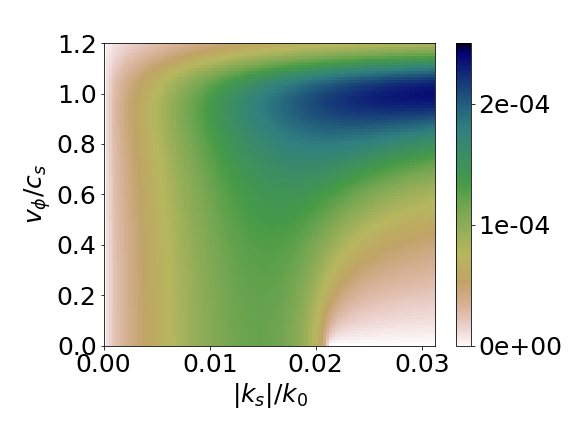
\includegraphics[width=0.25\textwidth]{G_Te1keV_Ti300_3e14_3w_1e-1nc_Hp.png}&
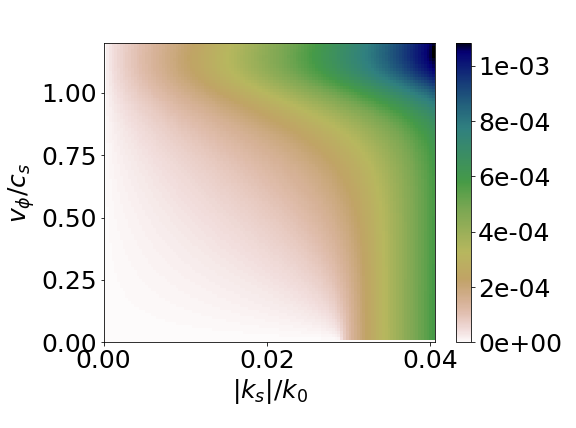
\includegraphics[width=0.25\textwidth]{k_Te1keV_Ti300_3e14_3w_1e-1nc_Hp.png}\\
(d) Fluid, $-\Im(k_{sx}/k_0)$  &
(e) Fluid, $\Re(k_{sx}/k_0)$  \\
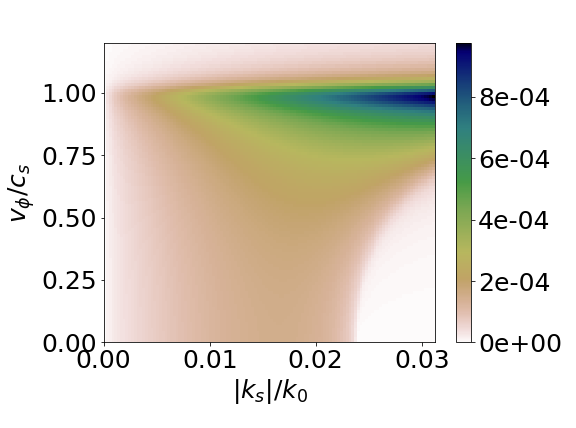
\includegraphics[width=0.25\textwidth]{Gf_Te1keV_Ti300_3e14_3w_1e-1nc_Hp.png}&
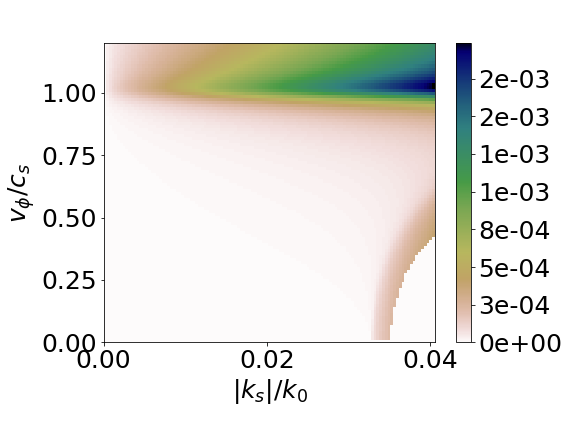
\includegraphics[width=0.25\textwidth]{kf_Te1keV_Ti300_3e14_3w_1e-1nc_Hp.png}
\end{tabular}
\caption{ \label{fig:dispe}  
Kinetic (a,b) and fluid (c,d) resolution of Eq. \eqref{eq:dispe2poly} for  $I_0 = 3\cdot 10^{14}\, \rm W.cm^{-2}$, $2\pi/k_0=0.35 \,\rm\mu m$, $T_e =1\,\rm  keV$, $ T_i=300\,  \rm eV$ in a H$^+$ and $n_{e0}=0.1n_c$.
 }
\end{figure}
\begin{figure}
\begin{tabular}{cc}
(a) Kinetic, $-\Im(k_{sx}/k_0)$ &
(b)  Kinetic, $\Re(k_{sx})$ \\
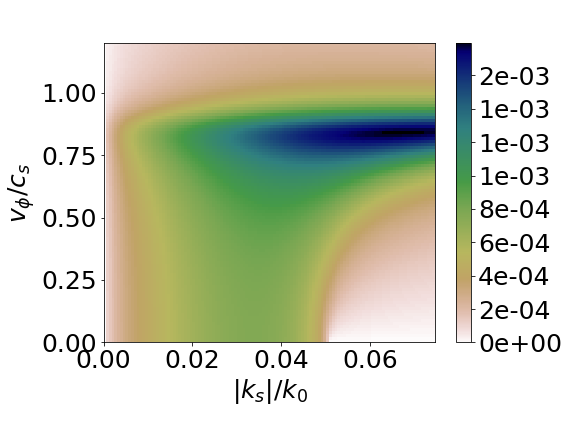
\includegraphics[width=0.25\textwidth]{G_Te700eV_Ti500_3e14_3w_1e-1nc_CH.png}&
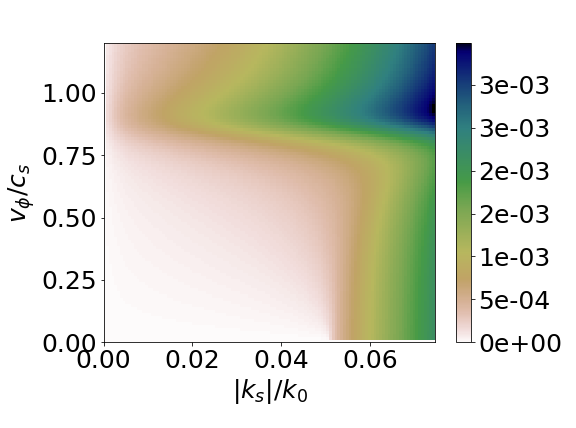
\includegraphics[width=0.25\textwidth]{k_Te700eV_Ti500_3e14_3w_1e-1nc_CH.png}\\
(d) Fluid, $-\Im(k_{sx}/k_0)$  &
(e) Fluid, $\Re(k_{sx}/k_0)$  \\
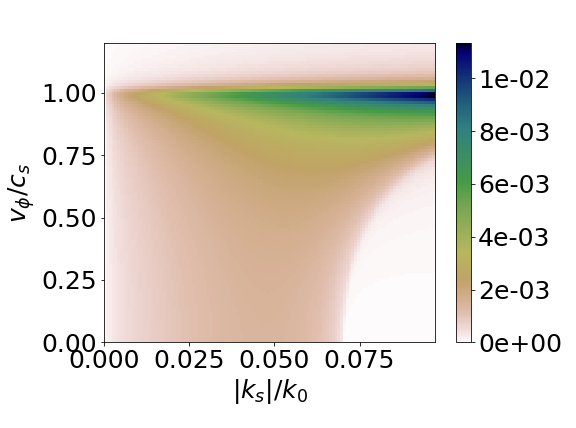
\includegraphics[width=0.25\textwidth]{Gf_Te700eV_Ti500_3e14_3w_1e-1nc_CH.png}&
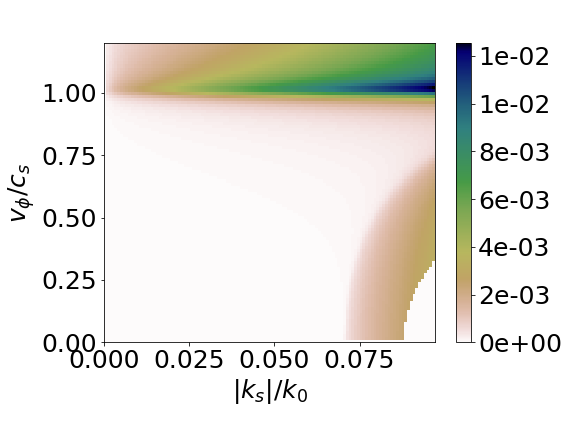
\includegraphics[width=0.25\textwidth]{kf_Te700eV_Ti500_3e14_3w_1e-1nc_CH.png}
\end{tabular}
\caption{ \label{fig:dispeCH}  
Kinetic (a,b) and fluid (c,d) resolution of Eq. \eqref{eq:dispe2poly} for  $I_0 = 3\cdot 10^{14}\, \rm W.cm^{-2}$, $2\pi/k_0=0.35 \,\rm\mu m$, for a CH plasma with $n_c=n_H$, $T_e =700\,\rm  eV$, $T_C=T_H =500\,  \rm eV$ and $n_{e0}=0.1n_c$. The value of the non-local correction [Eq. \eqref{eq:nl}], is obtained with the carbon parameters, corresponding to the smallest electron-ion mean-free-path. Use is made of the mean charge number, mean mass number   for calculating the sound speed and normalized Landau damping rate $c_s$ and $\gamma_0$.
 }
\end{figure}
Figures \ref{fig:dispe}(a-c)  illustrates the real and imaginary part of $k_{sx}/k_0$, solution of Eq. \eqref{eq:dispe2poly} as a function of the phase speed and of the wavevector amplitude, in both the kinetic (a,b) and fluid framework (c,d). The filamentation limit is recovered at $v_\phi=0$ and care has been taken to verify that, when $T_i\ll Z_iT_e$, both frameworks con\"incide. Moreover, in both calculations, $\Re[k_{sx}(v_\phi=0)]$ is vanishing as expected from the filamentation instability. As $v_\phi$ increases, one starts to enter in the forward Brillouin instability domain which peaks, for the mono-ion species case of Fig. \ref{fig:dispe}, around $(\vert k_s\vert/k_0, v_\phi/c_s) \simeq(0.03,1)$. Additionally, in both cases, the forward Brillouin spatial maximum  growth dominates the filamentation one. In the fluid framework, a much more peaked growth spectrum around  $ v_\phi/c_s\sim 1 $ is evidenced compared to the kinetic calculations. 

Interestingly, the kinetic calculation allows to consider multiple ion plasmas such as CH  illustrated in Fig. \ref{fig:dispeCH}. In the fluid framework, we are usually constrained to use the averaged-ion approximation, which gives in the case of the fourwad Brillouin, qualitatively different behavior as the spatial growth peaks at $v_\phi/c_s \simeq 0.75$ and $1$ for (a) and (b) respectively. 

For both Figs. \ref{fig:dispe} and \ref{fig:dispeCH}, from the kinetic framework ensues a  roughly twice smaller maximum growth rate than in the fluid framework. 

\section*{Acknowledgements}
%We also admit the role of the confinement following the COVID19 plague for forcing us to take the time to finalize this theoretical work. This work has been done under the auspices of CEA-DAM. 
% and the simulations were performed using HPC resources at TGCC/CCRT and CEA-DAM/TERA.
\bibliography{biblio}
\end{document}
